\section{Chess, Draughts and Naughts \& Crosses}

In the following sections a detailed analysis of the three games: Chess, Draughts, and Naughts \& Crosses will be performed. The reason for picking these three games in particular, is first of all the fact that none of the games includes dice, cards or other related objects, accept for it's pieces and a board. The second reason why we pick these three games is because they are among those we have biggest personal interest in. Therefore we want to dig deeper into the details of the components of these games (e.g. the pieces, the board, the squares etc.) to gain a better understanding of which features are needed in \productname. The respective history of the games and other related information will not be included in the analysis, since this has no relevans for gaining understandig of how our programming language could be designed.  

\subsection{Chess}
Chess is a board game of two oppenent players. It's a turn-based game which means one player makes a move, 
then the other player makes a move, then the first player makes a move and so on. Chess is played on a board of $8 \times 8$ squares. The squares are typically black and white, but can be any two colors (see figure \ref{fig:chess}). 
Each player has a total of 16 pieces: 8 pawns, 2 knights, 2 bishops, 2 rooks, a queen and a king. Each type of piece has unique ways to move. For instance a pawn can move only one square vertically forward or one square diagonal when capturing an enemy piece. 
A rook can move unlimited squares either forward or backward (vertical movement), or to the right or to the left (horisontal movement). 

Cut to the bone the game goes as follow: When a game starts the pieces are in their respective starting positions as seen in figure \ref{fig:chess}. The player with the white pieces always makes the first move, and after that the players shifts in turn in which clever moves are beeing taken and pieces are beeing captured until one player has checkmated the other - and the game is over. The checkmate situation is obtained when the king piece is in a position to be captured and cannot escape from capture \cite{chessrules}.

Special situation and moves. In chess there are a number of special situations and moves which doesn't follow the normal pattern in chess. Early we mentioned that a pawn can only move only one square vertically forward or one square diagonal when capturing an enemy piece. But this is not always true. If the pawn is in it's respective starting position it can move either one \textbf{or} two squares vertically forward. After moving from it's starting position it can only move one square forward the rest of the game. Another special move is the move called ``castling''. This move allows a player to move two pieces in one turn (the king and a rook).   

\begin{figure}
	\centering
		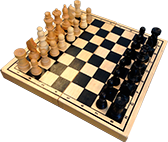
\includegraphics[scale=0.1]{pictures/chess.png}
		\caption{The board game chess with the pieces in start position.}
\label{fig:chess}
\end{figure}

\subsection{Naughts}

\subsection{Naughts \& Crosses}       